\documentclass[12pt]{book}
\usepackage[margin=.85in]{geometry} % for MARGIN
\usepackage[many]{tcolorbox}    	% for COLORED BOXES (tikz and xcolor included)


\usepackage{multicol}   
\usepackage{enumerate}
\usepackage[shortlabels]{enumitem}
\usepackage{varwidth}
\usepackage{tasks}
\usepackage[export]{adjustbox}
\usepackage[dvipsnames]{xcolor}

\usepackage{titleps}
\usepackage{setspace}               % for LINE SPACING
\usepackage[⟨options⟩]{fancyhdr}
\usepackage{enumitem}
\setlist{nosep}
\usepackage{tikz}
\usepackage{pgfplots}
\pgfplotsset{compat=1.5.1}
\usetikzlibrary{datavisualization}
\usetikzlibrary{datavisualization.formats.functions}

\newcommand{\D}{\displaystyle}


\setlength\parindent{0pt}   % killing indentation for all the text
\setstretch{1.3}            % setting line spacing to 1.3
\setlength\columnsep{0.25in} % setting length of column separator
\pagestyle{fancy}           % setting pagestyle to be headings

\usepackage[]{titlesec}

\fancyhead[L]{Math V04 - College Algebra}
\fancyhead[R]{Christina Papazacharioudakis}

\tcbset{
    sharp corners,
    colback = white,
    before skip = 0.2cm,    % add extra space before the box
    after skip = 0.5cm      % add extra space after the box
}                           % setting global options for tcolorbox

    \newtcolorbox{boxR}{
    fontupper = \color{black}, % font color
    boxrule = 1.5pt,
    colframe = black,
    rounded corners,
    arc = 5pt   % corners roundness
}

\definecolor{ballblue}{rgb}{0.13, 0.67, 0.8}

\begin{document}



\begin{comment}
Name: \underline{\hspace{100mm}}
\vspace{20mm}
  \centerline{\Large \textbf{Chapter 2: Equations and Inequalities} } 

{\large
\begin{center}
\begin{varwidth}{\textwidth}
\begin{enumerate}[2.1]
    \item The Regular Coordinate System and Graphs
    \item Linear Equations in One Variable
    \item Models and  Applications (Skipping)
    \item Complex Numbers
    \item Quadratic Equations
    \item Other Types of Equations
    \item Linear Inequalities and Absolute Value Inequalities
\end{enumerate}
\end{varwidth}
\end{center}

}
\newpage  
\end{comment}

\textbf{{\Large 3.4 Composition of Functions}}
\vspace{3mm}

Two functions $f$ and $g$ can be combined to form new functions $f+g$, $f-g$, $fg$, and $f/g$ in a similar way to the way we add, subtract, multiply, and divide real numbers.

\vspace{5mm}



\begin{boxR}
    \textbf{Sum, Difference, Product, and Quotient Functions}
    \vspace{1mm}
    \hline
    \vspace{2mm}
Given two functions $f$ and $g$, the following functions are defined as follows: 

\vspace{2mm}
\textbf{Sum Function:} $\D (f+g)(x)=f(x) + g(x)$
    \vspace{3mm}
    
\textbf{Difference Function:} $\D (f-g)(x)=f(x) - g(x)$
    \vspace{3mm}
    
\textbf{Product Function:}  $\D (fg)(x) = f(x)g(x)$
    \vspace{3mm}
    
    \textbf{Quotient Function:}
 $\D (f/g)(x) = \frac{f(x)}{g(x)} \hspace{3mm}, g(x)\neq 0$   


\end{boxR}


\underline{\textbf{Example 1 - Performing Algebraic Operations on Functions}}
\vspace{3mm}

Find and simplify the functions $(f-g)(x)$ and $(f/g)(x)$ given that $f(x)=x^2-1$ and $g(x)=x-1$.
\vspace{1mm}
\newpage

{\large \textbf{Create a Function by Composition of Functions}}

Performing algebraic operations on functions (adding, subtracting, multiplying, and dividing) created new functions. We can also create functions by composing them. This process includes taking the output of one function and using it as the input of another function. The resulting function is known as a \textbf{composite function}. We represent this combination by the following notation:
$$(f \circ g)(x) = f(g(x))$$
This reads ``$f$ of $g$ of $x$".
\\

For example, if $f(x) = x^2$ and $g(x)=x+2$ then,
\\

   $f(g(x))= $

   \vspace{50mm}




Note that in many cases, $f(g(x)) \neq g(f(x))$. They are different functions. Let's take a look:
\\

   $g(f(x))= $

   \vspace{50mm}

\newpage


\begin{boxR}
    \textbf{Composition of Functions}
    \vspace{1mm}
    \hline
    \vspace{2mm}
   When the output of one function is used as the input of another, we call the entire operation a composition of functions. This action defined a composite function, which we write as:
   $$ (f \circ g)(x) = f(g(x))$$

 The domain of $f \circ g$ is the set of all $x$ in the domain of $g$ such that $g(x)$ is also in the domain of $f$. 
\end{boxR}
{\large \textbf{Evaluating Composite Functions}}
\vspace{1mm}

Once we compose a new function from two existing functions, we need to be able to evaluate it for any input in its domain. We evaluate the inner function first, and then use its output as the input of the outer function.

\centerline{ 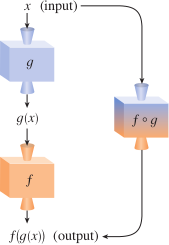
\includegraphics[scale=.9]{Chapter 3/3.4-figure1.png} }

\vspace{1mm}
\underline{\textbf{Example 5 - Using a Table to Evaluate a Composite Function}}

Find $f(g(3))$ and $g(f(3))$ using the table.
\\

\begin{tabular}{ |c|c|c| } 
 \hline
 $x$ & \hspace{3mm} $f(x) \hspace{3mm}$ & \hspace{3mm} $g(x)$ \hspace{3mm} \\
 \hline
 $1$ & $6$ & $3$ \\
 \hline
 $2$ & $8$ & $5$ \\
 \hline
 $3$ & $3$ & $2$ \\
 \hline
  $4$ & $1$ & $7$ \\
 \hline
\end{tabular}
\newpage


\textbf{Evaluating Composite Functions Using Graphs}



\begin{boxR}
    \textbf{How To}
    \vspace{1mm}
    \hline
    \vspace{2mm}
   \textbf{Given a composite function and graphs of its individual functions, evaluate it using the information provided by the graphs.}
   \begin{enumerate}
       \item Locate the given input to the inner function on the $x$-axis of its graph.
       \item Read off the output of the inner function from the  $y$-
       axis of its graph.
       \item Locate the inner function output on the $x$-axis of the graph of the outer function.
       \item Read the output of the outer function from the  $y$-axis of its graph. This is the output of the composite function.
   \end{enumerate}
\end{boxR}

  
\underline{\textbf{Example 6 - Using a Graph to Evaluate a Composite Function}}

Evaluate $f(g(1))$ and $g(f(2))$.
\\

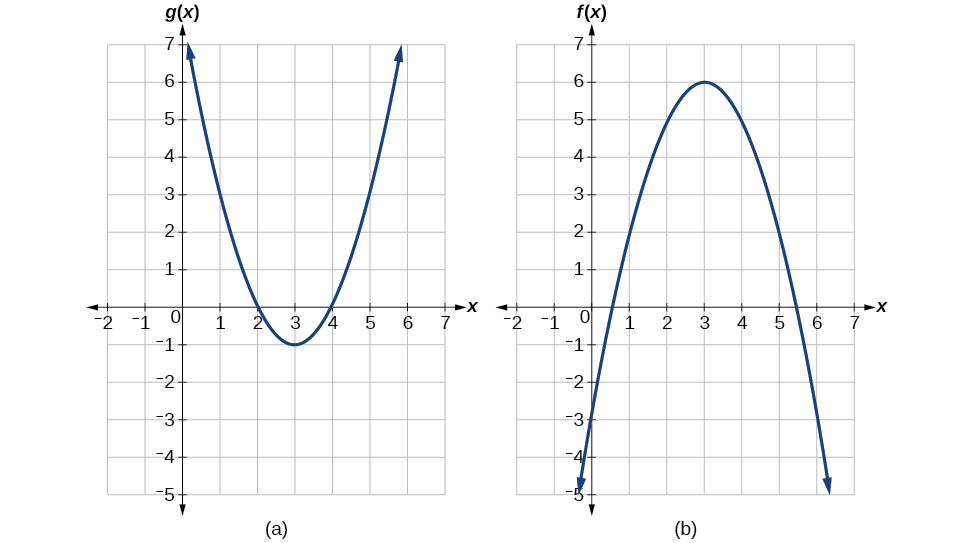
\includegraphics[scale=.8]{Chapter 3/3.4-figure2.jpeg}

 \newpage



{\large \textbf{Evaluating Composite Functions Using Formulas}}


When evaluating a composite function using formulas, the process of working from the inside out remains the same. 

\vspace{3mm}

\begin{boxR}
    \textbf{How To}
    \vspace{1mm}
    \hline
    \vspace{2mm}
    \textbf{Given a formula for a composite function, evaluate the function.}
    \begin{enumerate}
        \item Evaluate the inside function using the input value or variable provided.
        \item Use the resulting output as the input to the outside function.
    \end{enumerate}
\end{boxR}
\vspace{3mm}



\underline{\textbf{Example 7 - Evaluating a Composition of Functions Expressed as Formulas}}

Given $f(t)=t^2-t$ and $h(x)= 3x+2$, evaluate $f(h(1))$.

\newpage

{\large \textbf{Finding the Domain of a Composite Function}}

As mentioned in the beginning of this section, the domain of $f \circ g$ depends on both the domain of $g$ and the domain of $f$:
\\

\begin{boxR}
    \textbf{Domain of a Composite Function}
    \vspace{1mm}
    \hline
    \vspace{2mm}
    The domain of a composite function $f(g(x))$ is the set of those inputs $x$ in the domain of $g$ for which $g(x)$ is also in the domain of $f$.
\end{boxR}

\begin{boxR}
    \textbf{How To}
    \vspace{1mm}
    \hline
    \vspace{2mm}
    \textbf{Given a function composition $f(g(x))$ determine its domain.}
    \begin{enumerate}
        \item Find the domain of $g$.
        \item Find the domain of $f$
        \item Find the inputs $x$ in the domain of $g$ such that $g(x)$ is in the domain of $f$. That is, exclude $x$ values from the domain of $g$ for which $g(x)$ is not in the domain of $f$.
    \end{enumerate}
\end{boxR}

\underline{\textbf{Example 8 - Finding the Domain of a Composite Function}}
\vspace{2mm}

Find the domain of $(f \circ g)(x) = f(g(x))$ where 
$\D f(x) = \frac{5}{x-1}$ and $\D g(x) = \frac{4}{3x-2}$.

\newpage
{\large \textbf{Decomposing a Composite Function into its Component Functions}}
\vspace{3mm}

Given a composite function, we may want to write it as a composition of two simpler functions. Let's take a look:
\\

\underline{\textbf{Example 10 - Decomposing a Function}}
\vspace{2mm}

Write $\D h(x) = \sqrt{5-x^2}$ as the composition of two functions. 
\newpage






\end{document}


